\section{System Model}
\label{sec:system}

We evaluate a hybrid sidelink/optical link against the 3GPP TR~38.913 eV2X
reference row on a microscopic urban mobility model. Both media are exercised
on the same vehicle geometry, so the radio and optical paths available to a
given packet describe the same instant of the same world. Section~\ref{sec:sys:scenario}
describes the scenario, Section~\ref{sec:sys:rf} the sidelink resource model,
Section~\ref{sec:sys:vlc} the optical link, and Section~\ref{sec:sys:obs} what
a transmitter is permitted to observe. Parameters are listed in
Table~\ref{tab:params}.

\subsection{Scenario and Mobility}
\label{sec:sys:scenario}

Vehicles move on a one-way Manhattan grid of $6$ avenues spaced
\SI{244}{\metre} and $12$ cross streets spaced \SI{61}{\metre}, two lanes per
direction, illustrated in Fig.~\ref{fig:scene}. The asymmetric block ratio is
characteristic of the reference topology and is not incidental to the result:
it produces two distinct populations of communicating pairs, long runs along
avenues and short hops between cross streets, whose optical geometry differs
sharply.

All $40$ interior junctions are signalised on a fixed two-phase
\SI{45}{\second} cycle with staggered offsets. Vehicles follow a car-following
law with a \SI{2.5}{\metre} minimum standstill gap, draw from three classes
($90\%$ passenger car, $7\%$ van/SUV, $3\%$ bus/truck) at their configured body
dimensions, and enter at the boundary as a Poisson process tuned to hold one of
three target densities $\rho \in \{10, 20, 30\}$~veh/lane$\cdot$km. Traces
advance at \SI{50}{\milli\second} and are discarded for the first
\SI{300}{\second} so that the seeded formation disperses before measurement.

Signalisation matters for the optical link. The resulting traffic is
stop-and-go rather than free-flowing---median speed \SI{1.2}{\metre\per\second}
with roughly $38\%$ of vehicles stationary at any instant---so following pairs
hold short, stable separations for seconds at a time.


\begin{figure}[t]
  \centering
  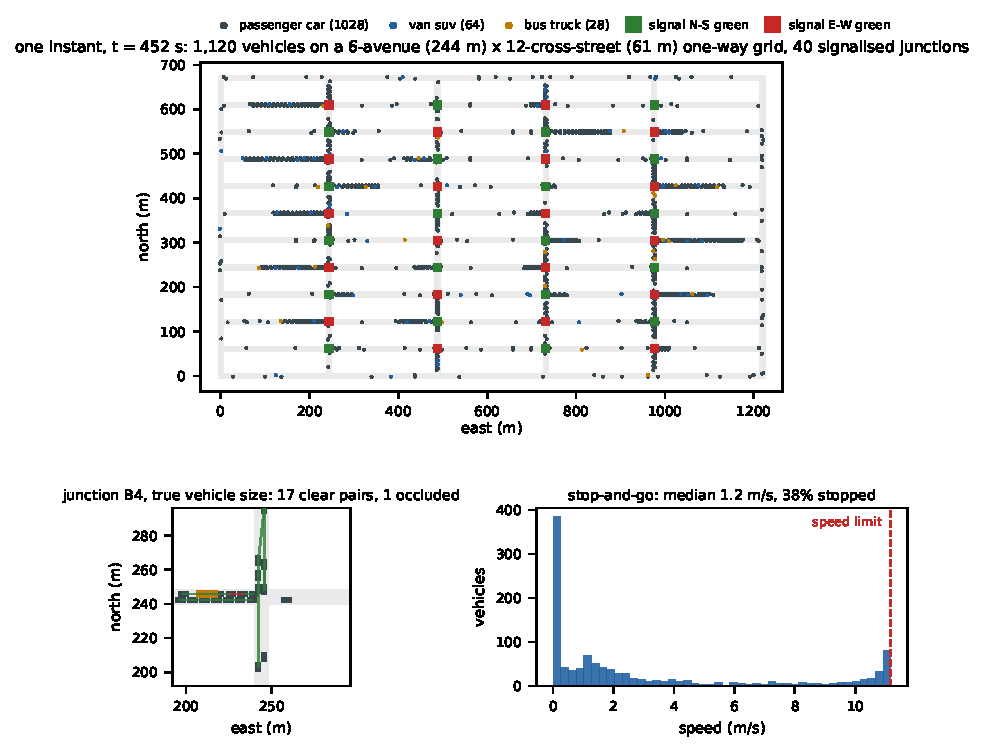
\includegraphics[width=\columnwidth]{figures/fig_traffic_scene.pdf}
  \caption{One instant of the scenario at $\rho = 30$: 1\,120 vehicles on the
  one-way grid with signal phases, and the speed distribution that follows from
  signalisation.}
  \label{fig:scene}
\end{figure}

\subsection{Sidelink Resource Model}
\label{sec:sys:rf}

The radio is NR-V2X mode~2 with sensing-based semi-persistent scheduling. A
vehicle senses the channel, excludes resources it observes to be reserved, and
selects from the remainder. We model the outcome of that procedure rather than
its signalling: a transmission fails when two vehicles select the same
resource, at a rate set by how many contenders there are and how reliably
sensing excludes them.

The quantity that governs the result is the size of the pool they select from.
With $S$ subchannels and a selection window of $W$ slots aligned to the
generation period, the pool offers
\begin{equation}
  M = S \, W
  \label{eq:pool}
\end{equation}
distinct (subchannel, slot) resources per period. For the profile of
Table~\ref{tab:params}, $M = 2 \times 200 = 400$.

Reliability on this link is bought with retransmissions. A packet granted $N$
blind attempts fails only if all $N$ are lost, so with per-attempt failure
probability $q$ and attempts drawn on distinct resources,
\begin{equation}
  p_{\mathrm{RF}} = q^{N}.
  \label{eq:rf}
\end{equation}
Each attempt, however, consumes one resource from the same pool that every
other vehicle draws from. With $n$ contenders in range each claiming $N$
attempts, the population asks for $nN$ of the $M$ that exist. We write this
claim as
\begin{equation}
  D = \frac{nN}{M},
  \label{eq:demand}
\end{equation}
and call the profile \emph{deliverable} only when $D \le 1$.

This is a supply constraint, not a performance one, and it is invisible to the
collision model itself. That model prices where one selection lands; it does
not ask whether every selection can be honoured simultaneously. A profile with
$D > 1$ therefore still reports an ordinary per-attempt failure probability and
a plausible miss rate, both of which describe an assignment that does not
exist. Every reliability figure in Section~\ref{sec:results} is reported
alongside its $D$ for this reason.

Sensing reliability is the one quantity the model declares it does not know
precisely. We carry it as a band---optimistic, nominal and pessimistic---rather
than a point value, and report the verdict on all three.

\subsection{Optical Link}
\label{sec:sys:vlc}

The optical link is vehicle-to-vehicle visible light between a leading
vehicle's tail lamps and a follower's photodiode, at \SI{0.55}{\metre} height
against a \SI{0.7}{\metre} emitter. The emission pattern is a modelled angular
intensity grid fitted so that every UN Regulation~112 Rev.4 Class~B
passing-beam limit is satisfied by construction; it is a regulatory
construction, not a measured lamp, and any optical figure quoted from it
inherits that.

Transmission is on-off keying at a \SI{5}{\mega\hertz} electrical bandwidth,
which is the optimistic edge of what automotive LED junction capacitance
supports. With rate-$1/4$ coding this puts \SI{2.4}{\milli\second} of airtime
on a \SI{300}{\byte} block---roughly five times the \SI{0.5}{\milli\second}
radio slot, a disparity that matters in Section~\ref{sec:results}.

An optical packet fails for one of three reasons: the receiver falls outside
the emitter's field of view, a third vehicle body occludes the path, or the
received signal is too weak for the coded threshold. The first two are
geometric and are decided by the same vehicle positions the radio model reads.
Occlusion is treated as complete: a body intersecting the line of sight
extinguishes the link rather than attenuating it. This is conservative for the
optical leg.

\subsection{Observability}
\label{sec:sys:obs}

Decisions and outcomes are deliberately separated. A transmitter chooses using
cooperative awareness messages---positions perturbed by
$\sigma = \SI{0.5}{\metre}$, delivered with \SI{50}{\milli\second} latency and
aged up to \SI{1}{\second}---while every reported miss rate is computed from
what the channel actually did. A policy that could not have been executed by a
vehicle is therefore visible as such, and Section~\ref{sec:results} states
explicitly which of its results are achievable and which are bounds.

\begin{table}[t]
  \centering
  \caption{Simulation parameters.}
  \label{tab:params}
  \small
  \begin{tabular}{@{}llr@{}}
    \toprule
    & Parameter & Value \\
    \midrule
    \multirow{6}{*}{\rotatebox{90}{Mobility}}
      & Avenues $\times$ cross streets & $6 \times 12$ \\
      & Spacing (avenue, cross street) & $244$, \SI{61}{\metre} \\
      & Lanes per direction & 2 \\
      & Speed limit & \SI{11.18}{\metre\per\second} \\
      & Signal cycle (fixed, two-phase) & \SI{45}{\second} \\
      & Densities $\rho$ & 10, 20, 30 veh/lane$\cdot$km \\
    \midrule
    \multirow{5}{*}{\rotatebox{90}{Sidelink}}
      & Subchannels $S$ & 2 \\
      & Selection window $W$ & 200 slots \\
      & Pool $M = SW$ & 400 per period \\
      & Slot airtime & \SI{0.5}{\milli\second} \\
      & Sensing reliability & 0.70 / 0.85 / 0.95 \\
    \midrule
    \multirow{4}{*}{\rotatebox{90}{Optical}}
      & Modulation & OOK, rate $1/4$ \\
      & Electrical bandwidth & \SI{5}{\mega\hertz} \\
      & Airtime (\SI{300}{\byte} block) & \SI{2.4}{\milli\second} \\
      & Receiver field of view & \SI{60}{\degree} \\
    \midrule
    \multirow{5}{*}{\rotatebox{90}{Service}}
      & Payload & \SI{300}{\byte} \\
      & Generation period & \SI{100}{\milli\second} \\
      & Deadline & \SI{3}{\milli\second} \\
      & Miss budget & $10^{-5}$ \\
      & RF attempts $N$ & 4 \\
    \midrule
    \multirow{3}{*}{\rotatebox{90}{Obs.}}
      & Position noise $\sigma$ & \SI{0.5}{\metre} \\
      & Track latency & \SI{50}{\milli\second} \\
      & Track lifetime & \SI{1}{\second} \\
    \bottomrule
  \end{tabular}
\end{table}
